\resizebox{0.8\textwidth}{!}{%
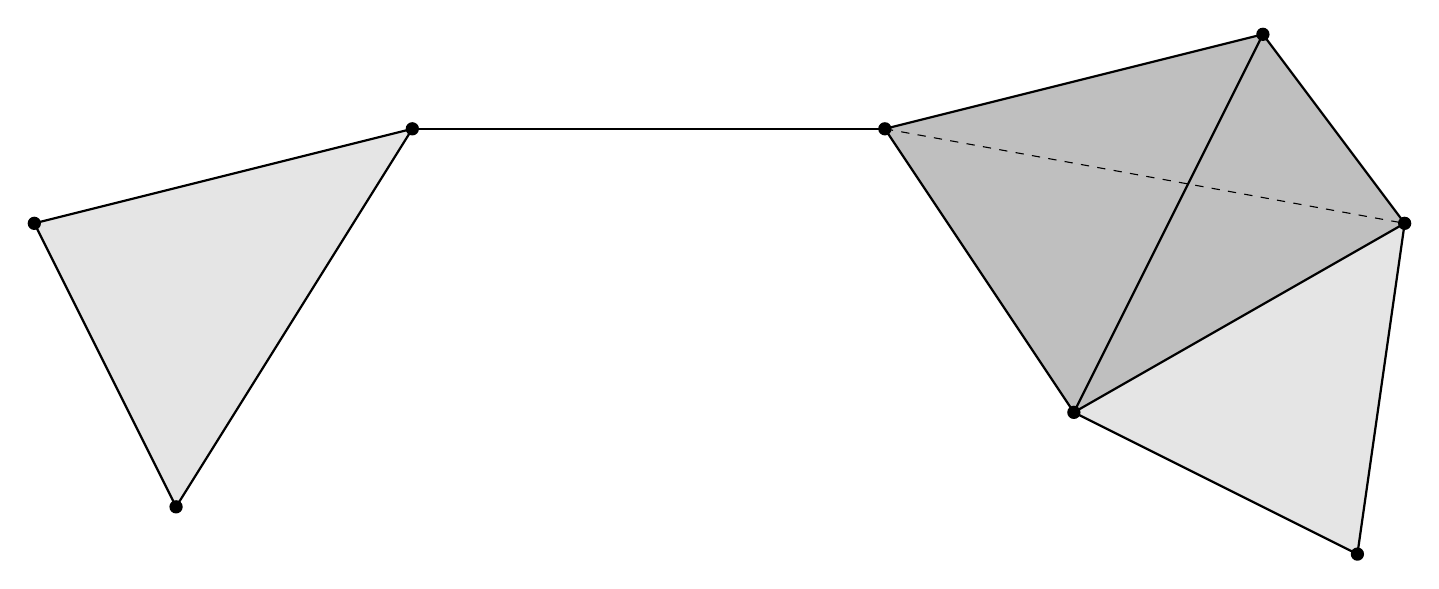
\begin{tikzpicture}[scale=1.2]

\begin{scope}[shift={(0,0)}]
        \coordinate (A) at (-3,0);
        \coordinate (B) at (2,0);
        \coordinate (C) at (-7,-1);
        \coordinate (D) at (-5.5,-4);
        \coordinate (E) at (6,1);
        \coordinate (F) at (4,-3);
        \coordinate (G) at (7.5,-1);
        \coordinate (H) at (7,-4.5);

        \fill[gray!20] (A) -- (C) -- (D) -- cycle;
        \fill[gray!20] (F) -- (G) -- (H) -- cycle;
        \fill[gray!50] (B) -- (E) -- (G) -- (F) -- cycle;
        
        \draw[thick] (A) -- (C) -- (D) -- cycle;
        \draw[thick] (B) -- (A);
        \draw[thick] (B) -- (E) -- (G) -- (F) --cycle;
        \draw[thick] (G) -- (H) -- (F);
        \draw[thick] (E) -- (F);
        \draw[dashed] (B) -- (G);
        
        % Wierzchołki
        \fill (A) circle[radius=2pt];% node[below] {$A$};
        \fill (B) circle[radius=2pt];% node[below] {$B$};
        \fill (C) circle[radius=2pt];% node[below] {$C$};
        \fill (D) circle[radius=2pt];% node[above] {$D$};
        \fill (E) circle[radius=2pt];% node[above] {$E$};
        \fill (F) circle[radius=2pt];% node[above] {$F$};
        \fill (G) circle[radius=2pt];% node[above] {$G$};
        \fill (H) circle[radius=2pt];% node[above] {$H$};
\end{scope}

\end{tikzpicture}
}